% Agent loop diagram — the canonical Ch 1 figure.
% Standalone TikZ source; compiled by `book-scaffold build-figures`
% (v4.2.0+) via pdflatex -> pdftocairo -> SVG.
\documentclass[tikz,border=4mm]{standalone}
\usepackage{tikz}
\usetikzlibrary{positioning, shapes.geometric, arrows.meta, calc}

\begin{document}
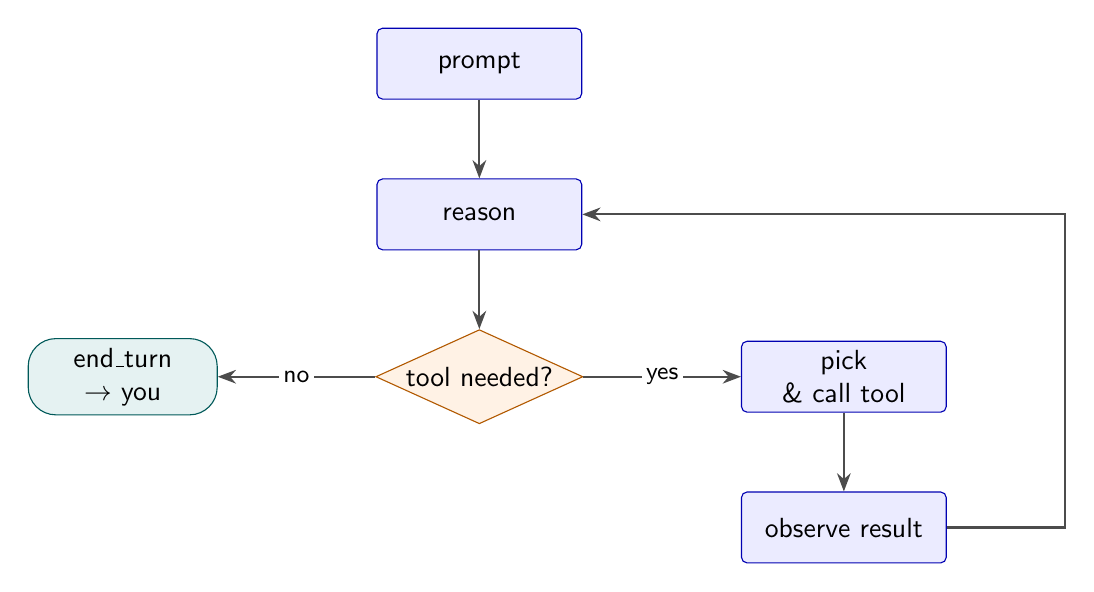
\begin{tikzpicture}[
  font=\sffamily,
  node distance=1cm and 1.5cm,
  box/.style={
    draw=blue!70!black, fill=blue!8, rounded corners=2pt,
    minimum width=2.6cm, minimum height=0.9cm, align=center
  },
  decision/.style={
    draw=orange!70!black, fill=orange!10,
    diamond, aspect=2.2, inner sep=1pt, align=center
  },
  endpoint/.style={
    draw=teal!70!black, fill=teal!10, rounded corners=10pt,
    minimum width=2.4cm, minimum height=0.9cm, align=center
  },
  arrow/.style={-Stealth, thick, draw=gray!60!black},
  arrowlabel/.style={font=\sffamily\small, fill=white, inner sep=1.5pt}
]

\node[box] (prompt) {prompt};
\node[box, below=of prompt] (reason) {reason};
\node[decision, below=of reason] (need) {tool needed?};
\node[box, right=2cm of need] (pick) {pick \\ \& call tool};
\node[box, below=of pick] (observe) {observe result};
\node[endpoint, left=2cm of need] (end) {end\_turn \\ $\to$ you};

\draw[arrow] (prompt) -- (reason);
\draw[arrow] (reason) -- (need);
\draw[arrow] (need) -- node[arrowlabel] {no} (end);
\draw[arrow] (need) -- node[arrowlabel] {yes} (pick);
\draw[arrow] (pick) -- (observe);
\draw[arrow] (observe.east) -| ++(1.5,0) |- (reason.east);

\end{tikzpicture}
\end{document}
